\chapter{Расчет биологической защиты}
\section{Описание реакторной установки}
Судовая реакторная установка КЛТ-40С представляет собой РУ с водоводянным реактором корпусного типа с гетерогенной частичной биологической защитой. 

На рисунке \ref{principle} представлена компоновка основного оборудования \nom{РУ}{реакторная установка} КЛТ-40С.
\begin{figure}[!h]
	\center
	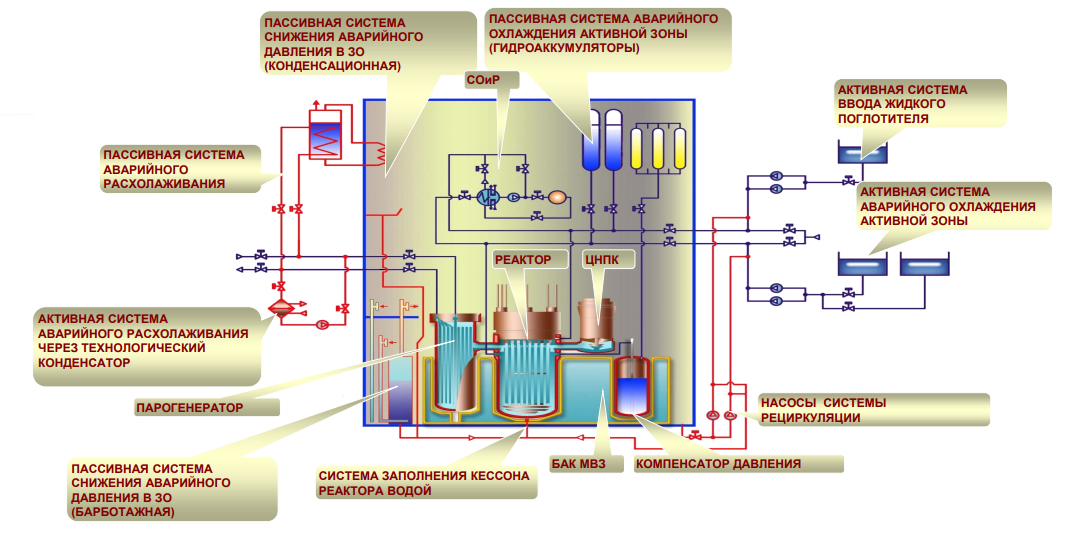
\includegraphics[height=8cm]{media/safe_2.png}
	\caption{Принципиальная схема РУ КЛТ-40С\cite{belyev}}
	\label{principle}
\end{figure}

На рисунке \ref{conctruction klt} представлена конструкция реактора КЛТ-40С.

\begin{figure}[!h]
	\center
	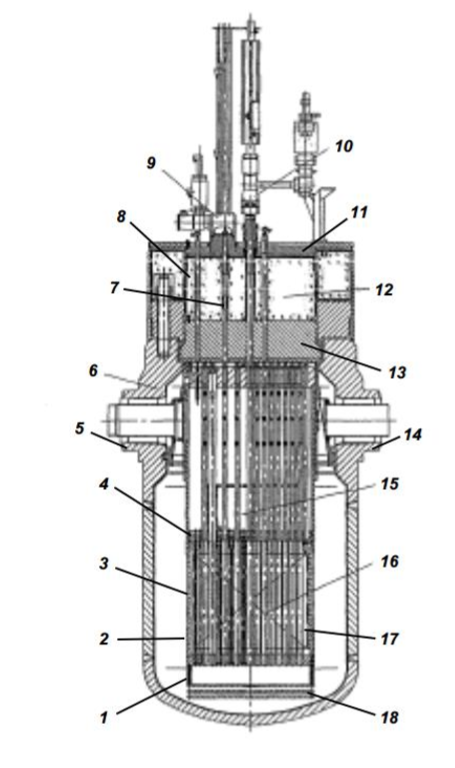
\includegraphics[height=13cm]{media/safe_3.png}
	\caption{Реактор КЛТ-40С:  1 – щелевой фильтр; 
		2 – обечайка; 
		3 – \nom{пэл}{поглощающий элемент}; 
		4 – \nom{РО}{рабочий орган} \nom{КГ}{компенсирующая группа}; 
		5 – патрубок парогенератора;  
		6 – корпус;  
		7 – стержни \nom{АЗ}{аварийная защита};  
		8 – биологическая защита; 
		9 – привод \nom{ИМ}{исполнительный механизм} АЗ; 
		10 – привод ИМ КГ; 
		11 – верхняя плита;  
		12 – крышка; 
		13 – силовая плита; 
		14 – патрубок \nom{ЦНПК}{циркуляционный насос первого контура };  
		15 – выемной блок;  
		16 – активная зона; 
		17 – \nom{ТВС}{тепловыделяющая сборка}; 
		18 – донные экраны \cite{deev}}
	\label{conctruction klt}
\end{figure}

Корпус реактора состоит из эллиптического днища, обечайки с патрубками находящейся в верхней части, и нижней цилиндрической обечайки. Корпус состоит из высокопрочной перлитной стали, изнутри защищен от коррозии нержавеющей герметичной облицовкой. Крышка, закрывающая корпус сверху, представляет собой плоскую силовую плиту. Она прижимается к верхней части корпуса фланцем с крепежным оборудованием. Биологическая защита располагается между верхней и силовой плитами и состоит из серпентинитового бетона.

К нижней плите крепится щелевой фильтр с экранами, который не допускает попадания в активную зону посторонних предметов. Экраны служат для уменьшения нейтронного потока на днище корпуса реактора. 

Активная зона находится внутри корпуса реактора, где располагается выемной блок. Вокруг активной зоны находится отражатель,представляющий собой слой воды и стальных боковых экранов, снижающий уровень воздействующего на корпус нейтронного и гамма-излучения из активной зоны. Сам же корпус реактора помещен в бак металловодной защиты.

Бак металловодной защиты - емкость, наполненная водой. В баке размещены стальные листы, чтобы ослабить воздействие быстрых нейтронов и гамма-излучения. Размеры бака определяются из условий обеспечения необходимого уровня ослабления излучений. 

\section{Постановка задачи}
Рассчитать минимальный размер биологической защиты реактора, обеспечивающий радиационную безопасность обслуживающего персонала.

\section{Построение одномерной геометрической модели биологической защиты}

Расчетная композиция биологической защиты приведена на рисунке \ref{composition}.

\begin{figure}[!h]
	\center
	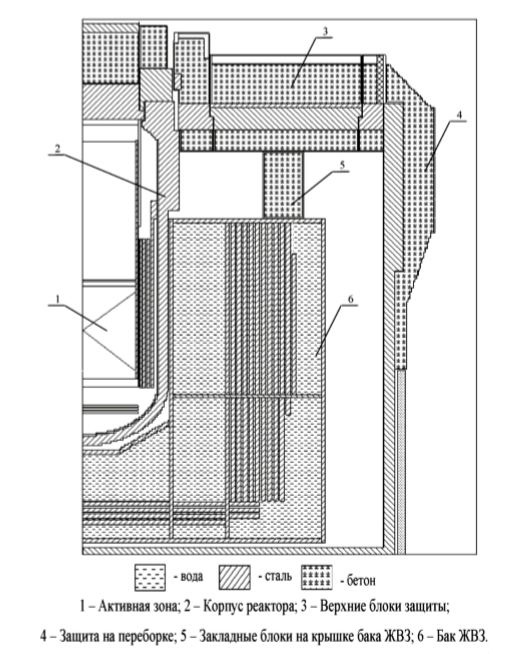
\includegraphics[height=16cm]{media/safe_4.png}
	\caption{Состав композиции\cite{andreev}}
	\label{composition}
\end{figure}
Рассмотрим схему атомной подводной лодки \ref{chema apl}. Уровень радиации будем рассчитывать в секторе жилые помещения(Ж).
\begin{figure}[!h]
	\center
	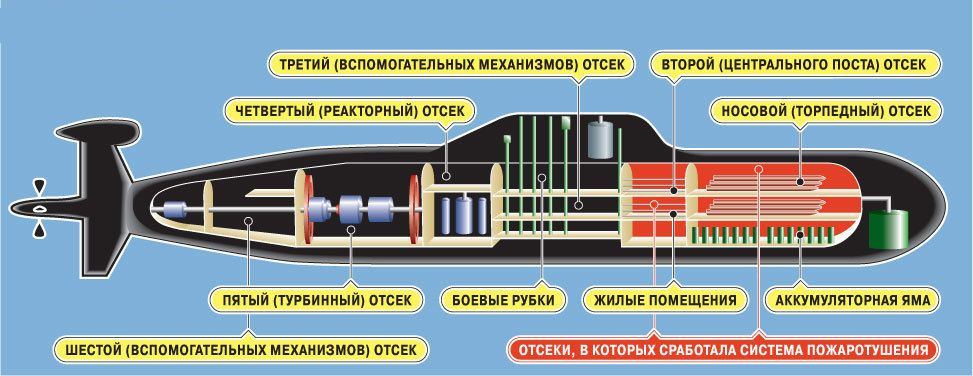
\includegraphics[height=6.3cm]{media/safe_5.png}
	\caption{Схема АПЛ}
	\label{chema apl}
\end{figure}

На основе представленного состава биологической защиты и схемы атомной подводной лодки построим одномерную геометрическую модель биологической защиты. В данной модели мы пренебрегаем слоем воздуха, так как он является плохим радиационно-защитным материалом. В таблице \ref{par_protec} приведены параметры слоев биологической защиты.
\begin{figure}[!h]
	\center
	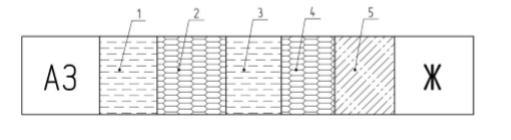
\includegraphics[height=5cm]{media/safe_6.png}
	\caption{Одномерная геометрическая модель биологической защиты}
\end{figure}

\begin{table}[!h]
\caption{ Параметры слоев защиты}
\label{par_protec}
\begin{tabular}{|c| c| c| c| c|}\hline
\textnumero & Защитный слой & Материал & Размер,см & Плотность, г/см$^3$\\ \hline	
1 & Отражатель & Вода & 30 & 0.7\\ \hline
2 & Корпус реактора & Сталь & 15 & 7.8\\ \hline
3 & Вода в \nom{МВЗ}{металловодная защита} & Вода & 150 & 1\\ \hline
4 & Стенки, стальные листы МВЗ & Сталь & 52.4 & 7.8\\ \hline
5 & Бетонная периферийная  & Бетон & Надо & 2.4\\ 
 & биологическая защита & & определить & \\ \hline
\end{tabular}
\end{table}
